\documentclass[titlepage]{ltjsbook}
\usepackage[
  paperheight=232truemm, paperwidth=182truemm,
  top=20truemm, bottom=15truemm, inner=15truemm, outer=15truemm
  ]{geometry}

%\documentclass[tombow, paper={182truemm, 232truemm}, titlepage]{ltjsbook}
\usepackage{amsmath}
\usepackage{amsfonts}
\usepackage{textgreek}
\usepackage[luatex]{graphicx} 
\usepackage[svgnames]{xcolor}
\usepackage{sty/julia-syntax-highlighting} % 
\usepackage[export]{adjustbox} % added

\usepackage{fancyhdr}
\pagestyle{fancy}

\newcommand{\jl}{\lstinline[language=julia]}

\title{\Huge \textbf{Juliaで学ぶ計算論的神経科学}}
\author{\huge 山本 拓都}
\date{\huge \today} 
\begin{document}
\maketitle

\setcounter{tocdepth}{2}
\tableofcontents
\clearpage

%\part{}
\chapter{局所学習則}
\section{自己組織化マップと視覚野の構造}
視覚野にはコラム構造が存在する.こうした構造は神経活動依存的な発生  (activity dependent development) により獲得される.本節では視覚野のコラム構造を生み出す数理モデルの中で,\textbf{自己組織化マップ (self-organizing map)}\index{じこそしきかまっぷ (self-organizing map)@自己組織化マップ (self-organizing map)} \citep{Kohonen1982-mn}, \citep{Kohonen2013-yt}を取り上げる.

自己組織化マップを視覚野の構造に適応したのは\citep{Obermayer1990-gq} \citep{N_V_Swindale1998-ri}などの研究である.視覚野マップの数理モデルとして自己組織化マップは受容野を考慮しないなどの簡略化がなされているが,単純な手法にして視覚野の構造に関する良い予測を与える.他の数理モデルとしては自己組織化マップと発想が類似している \textbf{Elastic net}\index{Elastic net}  \citep{Durbin1987-bp} \citep{Durbin1990-xx} \citep{Carreira-Perpinan2005-gy} (ここでのElastic netは正則化手法としてのElastic net regularizationとは異なる)や受容野を明示的に設定した \citep{Tanaka2004-vz}, \citep{Ringach2007-oe}などのモデルがある.総説としては\citep{Das2005-mq},\citep{Goodhill2007-va} ,数理モデル同士の関係については\citep{2002-nm}が詳しい.

自己組織化マップでは「抹消から中枢への伝達過程で損失される情報量」,および「近い性質を持ったニューロン同士が結合するような配線長」の両者を最小化するような学習が行われる.包括性 (coverage) と連続性 (continuity) のトレードオフとも呼ばれる \citep{Carreira-Perpinan2005-gy}  (Elastic netは両者を明示的に計算し,線形結合で表されるエネルギー関数を最小化する.Elastic netは本書では取り扱わないが,MATLAB実装が公開されている
\url{https://faculty.ucmerced.edu/mcarreira-perpinan/research/EN.html}) . 連続性と関連する事項として,近い性質を持つ細胞が脳内で近傍に存在する現象があり,これを\textbf{トポグラフィックマッピング (topographic mapping)}\index{とぽぐらふぃっくまっぴんぐ (topographic mapping)@トポグラフィックマッピング (topographic mapping)} と呼ぶ.トポグラフィックマッピングの数理モデルの初期の研究としては\citep{Von_der_Malsburg1973-bz} \citep{Willshaw1976-zo} \citep{Takeuchi1979-mi}などがある.

発生の数理モデルに関する総説 \citep{Van_Ooyen2011-fz}, \citep{Goodhill2018-ho}
\subsection{単純なデータセット}
SOMにおける$n$番目の入力を $\mathbf{v}(t)=\mathbf{v}_n\in \mathbb{R}^{D} (n=1, \ldots, N)$,$m$番目のニューロン$ (m=1, \ldots, M) $の重みベクトル (または活動ベクトル, 参照ベクトル) を$\mathbf{w}_m(t)\in \mathbb{R}^{D}$とする \citep{Kohonen2013-yt}.また,各ニューロンの物理的な位置を$\mathbf{x}_m$とする.このとき,$\mathbf{v}(t)$に対して$\mathbf{w}_m(t)$を次のように更新する.

まず,$\mathbf{v}(t)$と$\mathbf{w}_m(t)$の間の距離が最も小さい (類似度が最も大きい) ニューロンを見つける.距離や類似度としてはユークリッド距離やコサイン類似度などが考えられる.


\begin{align}
&[\text{ユークリッド距離}]: c = \underset{m}{\operatorname{argmin}}\left[\|\mathbf{v}(t)-\mathbf{w}_m(t)\|^2\right]\\
&[\text{コサイン類似度}]: c  = \underset{m}{\operatorname{argmax}}\left[\frac{\mathbf{w}_m(t)^\top\mathbf{v}(t)}{\|\mathbf{w}_m(t)\|\|\mathbf{v}(t)\|}\right]
\end{align}


この,$c$番目のニューロンを\textbf{勝者ユニット(best matching unit; BMU)}\index{しょうしゃゆにっと(best matching unit; BMU)@勝者ユニット(best matching unit; BMU)} と呼ぶ.コサイン類似度において,$\mathbf{w}_m(t)^\top\mathbf{v}(t)$は線形ニューロンモデルの出力となる.このため,コサイン距離を採用する方が生理学的に妥当でありSOMの初期の研究ではコサイン類似度が用いられている \citep{Kohonen1982-mn}.しかし,コサイン類似度を用いる場合は$\mathbf{w}_m$および$\mathbf{v}$を正規化する必要がある.ユークリッド距離を用いると正規化なしでも学習できるため,SOMを応用する上ではユークリッド距離が採用される事が多い.ユークリッド距離を用いる場合,$\mathbf{w}_m$は重みベクトルではなくなるため,活動ベクトルや参照ベクトルと呼ばれる.ここでは結果の安定性を優先してユークリッド距離を用いることとする.

こうして得られた$c$を用いて$\mathbf{w}_m$を次のように更新する.


\begin{equation}
\mathbf{w}_m(t+1)=\mathbf{w}_m(t)+h_{cm}(t)[\mathbf{v}(t)-\mathbf{w}_m(t)]
\end{equation}


ここで$h_{cm}(t)$は近傍関数 (neighborhood function) と呼ばれ,$c$番目と$m$番目のニューロンの距離が近いほど大きな値を取る.ガウス関数を用いるのが一般的である.


\begin{equation}
h_{cm}(t)=\alpha(t)\exp\left(-\frac{\|\mathbf{x}_c-\mathbf{x}_m\|^2}{2\sigma^2(t)}\right)
\end{equation}


ここで$\mathbf{x}$はニューロンの位置を表すベクトルである.また,$\alpha(t), \sigma(t)$は単調に減少するように設定する.\footnote{Generative topographic map (GTM)を用いれば$\alpha(t), \sigma(t)$の縮小は必要ない.また,SOMとGTMの間を取ったモデルとしてS-mapがある.}
\lstinputlisting[language=julia]{./text/local-learning-rule/self-organizing-map/002.jl}
ToDo: dimsをv, wで修正
\lstinputlisting[language=julia]{./text/local-learning-rule/self-organizing-map/004.jl}
\lstinputlisting[language=julia]{./text/local-learning-rule/self-organizing-map/005.jl}
\lstinputlisting[language=julia]{./text/local-learning-rule/self-organizing-map/006.jl}
\lstinputlisting[language=julia]{./text/local-learning-rule/self-organizing-map/007.jl}
近傍関数 (neighborhood function)のための二次元ガウス関数を実装する.Winnerニューロンからの距離に応じて値が減弱する関数である.ここでは一つの入力に対して全てのニューロンの活動ベクトルを更新するということはせず,winner neuronの近傍のニューロンのみ更新を行う.つまり,更新においてはglobalではなくlocalな処理のみを行うということである  (Winner neuronの決定にはWTAによるglobalな評価が必要ではあるが) .
自己組織化マップのメインとなる関数を書く.ナイーブに実装する.この方法だと空間が円,球体やトーラスのように周期性を持つ場合にも適応できる.
\lstinputlisting[language=julia]{./text/local-learning-rule/self-organizing-map/010.jl}
今回のように2次元のみを扱う場合はwinner neuronの周辺だけをsliceで抜き出して重み更新する方が高速である.
\lstinputlisting[language=julia]{./text/local-learning-rule/self-organizing-map/012.jl}
\lstinputlisting[language=julia]{./text/local-learning-rule/self-organizing-map/013.jl}
\lstinputlisting[language=julia]{./text/local-learning-rule/self-organizing-map/014.jl}
青点が$\mathbf{v}$,オレンジの点が$\mathbf{w}$である.黒線はニューロン間の位置関係を表す (これはWeight unfolding diagramsと呼ばれる).下段のヒートマップは$\mathbf{w}$の一番目の次元を表す.学習が進むとともに近傍のニューロンが近い活動ベクトルを持つことがわかる.
\lstinputlisting[language=julia]{./text/local-learning-rule/self-organizing-map/016.jl}
\lstinputlisting[language=julia]{./text/local-learning-rule/self-organizing-map/017.jl}
\begin{figure}[ht]
	\centering
	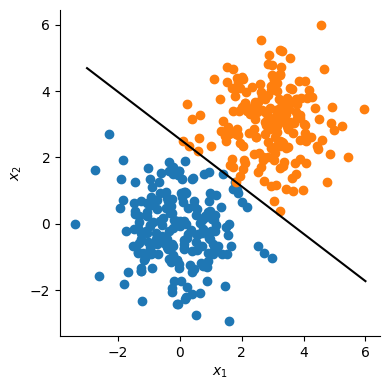
\includegraphics[scale=0.8, max width=\linewidth]{./fig/local-learning-rule/logistic-regression-perceptron/cell017.png}
	\caption{cell017.png}
	\label{cell017.png}
\end{figure}
unified distance matrixを描画する.隣接する要素とは位置の差の絶対値が1であることを利用する.
\lstinputlisting[language=julia]{./text/local-learning-rule/self-organizing-map/019.jl}
\lstinputlisting[language=julia]{./text/local-learning-rule/self-organizing-map/020.jl}
\lstinputlisting[language=julia]{./text/local-learning-rule/self-organizing-map/021.jl}
\lstinputlisting[language=julia]{./text/local-learning-rule/self-organizing-map/022.jl}
複数の点が同じ位置に重なっていることに注意.
\lstinputlisting[language=julia]{./text/local-learning-rule/self-organizing-map/024.jl}
\begin{figure}[ht]
	\centering
	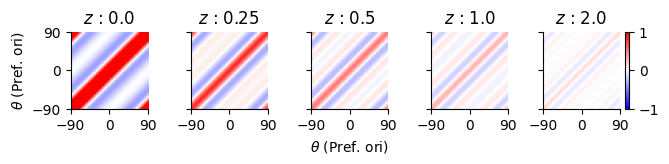
\includegraphics[scale=0.8, max width=\linewidth]{./fig/bayesian-brain/neural-sampling/cell024.png}
	\caption{cell024.png}
	\label{cell024.png}
\end{figure}
\subsection{視覚野マップ}
集合の直積を配列として返す関数 \jl{product}と極座標を直交座標に変換する関数 \jl{pol2cart}を用意する.
\lstinputlisting[language=julia]{./text/local-learning-rule/self-organizing-map/026.jl}
刺激と初期の活動ベクトルは\citep{Carreira-Perpinan2005-gy} を参考に作成.直積\jl{product}で全ての組の入力を作成する.
\lstinputlisting[language=julia]{./text/local-learning-rule/self-organizing-map/028.jl}
\lstinputlisting[language=julia]{./text/local-learning-rule/self-organizing-map/029.jl}
\lstinputlisting[language=julia]{./text/local-learning-rule/self-organizing-map/030.jl}
描画用関数を実装する. \jl{w_history}を用いてアニメーションを作成すると発達の過程が可視化されるが,これは読者への課題とする.
\lstinputlisting[language=julia]{./text/local-learning-rule/self-organizing-map/032.jl}
\lstinputlisting[language=julia]{./text/local-learning-rule/self-organizing-map/033.jl}
\begin{figure}[ht]
	\centering
	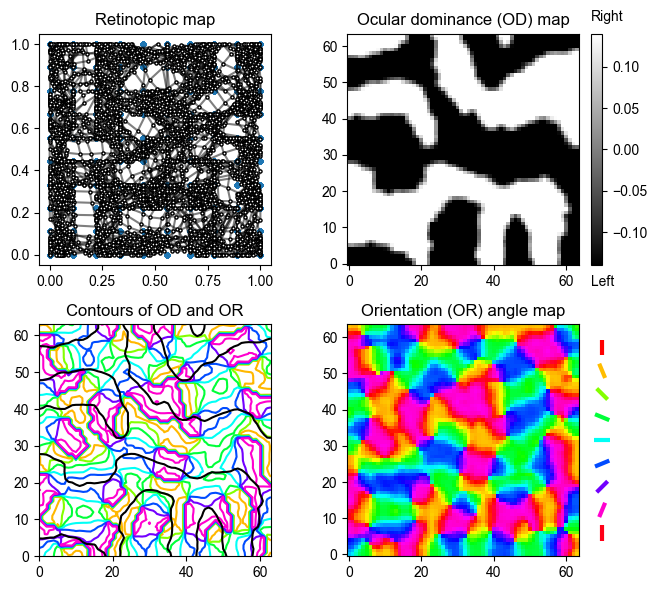
\includegraphics[scale=0.8, max width=\linewidth]{./fig/local-learning-rule/self-organizing-map/cell033.png}
	\caption{cell033.png}
	\label{cell033.png}
\end{figure}


\chapter{神経回路網によるベイズ推論}
\section{確率的集団符号化 (probabilistic population coding)}
Distributional Population Coding or distributed distributional codes (DDCs)
ポアソン分布
\begin{equation}
P(X=k)={\frac  {e^{-\lambda} \lambda^k}{k!}}
\end{equation}
より,
\begin{equation}
p(y \mid \mathbf{x}) \propto \prod_{i} \frac{e^{-f_{i}(y)} f_{i}(y)^{x_{i}}}{x_{i} !} p(y)
\end{equation}

\section{マルコフ連鎖モンテカルロ法 (MCMC)}
前節では解析的に事後分布の計算をした.事後分布を近似的に推論する方法の1つに\textbf{\index{まるこふれんさもんてかるろほう (Markov chain Monte Carlo methods; MCMC)@マルコフ連鎖モンテカルロ法 (Markov chain Monte Carlo methods; MCMC)}} がある.他の近似推論の手法としてはLaplace近似や変分推論 (variational inference) などがある.MCMCは他の手法に比して,事後分布の推論だけでなく,確率分布を神経活動で表現する方法を提供するという利点がある.

\footnote{
変分推論は入れた方がいいと思うが,紙幅の都合上いれられるか微妙である.
}

データを$X$とし,パラメータを$\theta$とする.


\begin{equation}
p(\theta\mid X)=\frac{p(X\mid \theta)p(\theta)}{\int p(X\mid \theta)p(\theta)d\theta}
\end{equation}


分母の積分計算$\int p(X\mid \theta)p(\theta)d\theta$が求まればよい.

\subsubsection{モンテカルロ法}

\subsubsection{マルコフ連鎖}
\subsection{Metropolis-Hastings法}
\lstinputlisting[language=julia]{./text/bayesian-brain/mcmc/002.jl}
\lstinputlisting[language=julia]{./text/bayesian-brain/mcmc/003.jl}
\lstinputlisting[language=julia]{./text/bayesian-brain/mcmc/004.jl}
\begin{figure}[ht]
	\centering
	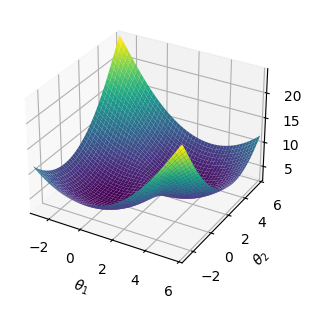
\includegraphics[scale=0.8, max width=\linewidth]{./fig/bayesian-brain/mcmc/cell004.png}
	\caption{cell004.png}
	\label{cell004.png}
\end{figure}
\lstinputlisting[language=julia]{./text/bayesian-brain/mcmc/005.jl}
\lstinputlisting[language=julia]{./text/bayesian-brain/mcmc/006.jl}
\lstinputlisting[language=julia]{./text/bayesian-brain/mcmc/007.jl}
\lstinputlisting[language=julia]{./text/bayesian-brain/mcmc/008.jl}
\lstinputlisting[language=julia]{./text/bayesian-brain/mcmc/009.jl}
\begin{figure}[ht]
	\centering
	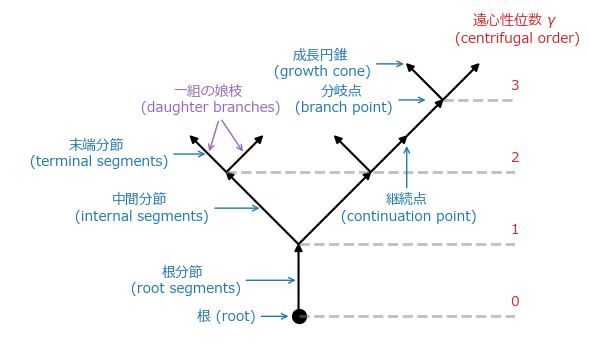
\includegraphics[scale=0.8, max width=\linewidth]{./fig/neuron-model/neurite-growth-model/cell009.png}
	\caption{cell009.png}
	\label{cell009.png}
\end{figure}
\subsection{ランジュバン・モンテカルロ法 (LMC)}
拡散過程


\begin{equation}
{\frac{d\theta}{dt}}=\nabla \log p (\theta)+{\sqrt 2}{d{W}}
\end{equation}


Euler–Maruyama法により,
\lstinputlisting[language=julia]{./text/bayesian-brain/mcmc/011.jl}
\lstinputlisting[language=julia]{./text/bayesian-brain/mcmc/012.jl}
\lstinputlisting[language=julia]{./text/bayesian-brain/mcmc/013.jl}
\lstinputlisting[language=julia]{./text/bayesian-brain/mcmc/014.jl}
\begin{figure}[ht]
	\centering
	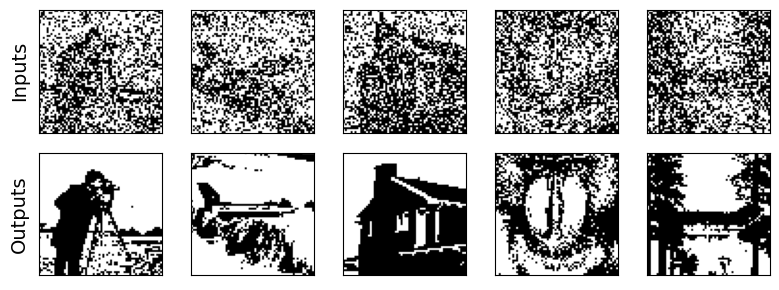
\includegraphics[scale=0.8, max width=\linewidth]{./fig/energy-based-model/hopfield-model/cell014.png}
	\caption{cell014.png}
	\label{cell014.png}
\end{figure}
\subsection{ハミルトニアン・モンテカルロ法 (HMC法)}
ハミルトニアン・モンテカルロ法(Hamiltonian Monte Calro)あるいはハイブリッド・モンテカルロ法(Hybrid Monte Calro)という

一般化座標を$\mathbf{q}$, 一般化運動量を$\mathbf{p}$とする.ポテンシャルエネルギーを$U(\mathbf{q})$としたとき,古典力学 (解析力学) において保存力のみが作用する場合の\textbf{\index{はみるとにあん (Hamiltonian)@ハミルトニアン (Hamiltonian)}} $\mathcal{H}(\mathbf{q}, \mathbf{p})$は


\begin{equation}
\mathcal{H}(\mathbf{q}, \mathbf{p})\triangleqU(\mathbf{q})+\frac{1}{2}\|\mathbf{p}\|^2
\end{equation}


となる.このとき,次の2つの方程式が成り立つ.


\begin{equation}
\frac{d\mathbf{q}}{dt}=\frac{\partial \mathcal{H}}{\partial \mathbf{p}}=\mathbf{p},\quad\frac{d\mathbf{p}}{dt}=-\frac{\partial \mathcal{H}}{\partial \mathbf{q}}=-\frac{\partial U}{\partial \mathbf{q}}
\end{equation}


これを\textbf{\index{はみるとんのうんどうほうていしき(hamilton's equations of motion)@ハミルトンの運動方程式(hamilton's equations of motion)}} あるいは\textbf{\index{せいじゅんほうていしき (canonical equations)@正準方程式 (canonical equations)}} という.


この処理をMetropolis-Hastings法における採用・不採用アルゴリズムという.

リープフロッグ(leap frog)法により離散化する.
\lstinputlisting[language=julia]{./text/bayesian-brain/mcmc/016.jl}
\lstinputlisting[language=julia]{./text/bayesian-brain/mcmc/017.jl}
\lstinputlisting[language=julia]{./text/bayesian-brain/mcmc/018.jl}
\lstinputlisting[language=julia]{./text/bayesian-brain/mcmc/019.jl}
\lstinputlisting[language=julia]{./text/bayesian-brain/mcmc/020.jl}
\begin{figure}[ht]
	\centering
	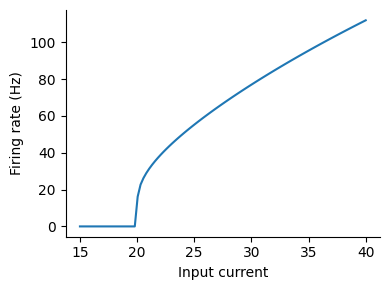
\includegraphics[scale=0.8, max width=\linewidth]{./fig/neuron-model/lif/cell020.png}
	\caption{cell020.png}
	\label{cell020.png}
\end{figure}
*ToDo: 自己相関確認する*
\subsection{線形回帰への適応}
\lstinputlisting[language=julia]{./text/bayesian-brain/mcmc/023.jl}
\lstinputlisting[language=julia]{./text/bayesian-brain/mcmc/024.jl}
\lstinputlisting[language=julia]{./text/bayesian-brain/mcmc/025.jl}
\lstinputlisting[language=julia]{./text/bayesian-brain/mcmc/026.jl}
\lstinputlisting[language=julia]{./text/bayesian-brain/mcmc/027.jl}
\lstinputlisting[language=julia]{./text/bayesian-brain/mcmc/028.jl}
\lstinputlisting[language=julia]{./text/bayesian-brain/mcmc/029.jl}
\lstinputlisting[language=julia]{./text/bayesian-brain/mcmc/030.jl}
\begin{figure}[ht]
	\centering
	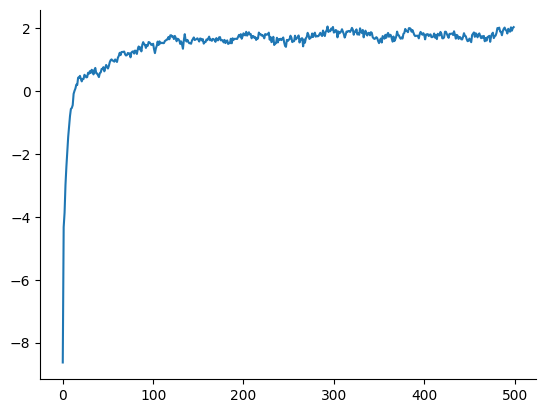
\includegraphics[scale=0.8, max width=\linewidth]{./fig/bayesian-brain/mcmc/cell030.png}
	\caption{cell030.png}
	\label{cell030.png}
\end{figure}
\lstinputlisting[language=julia]{./text/bayesian-brain/mcmc/031.jl}
\lstinputlisting[language=julia]{./text/bayesian-brain/mcmc/032.jl}
\begin{figure}[ht]
	\centering
	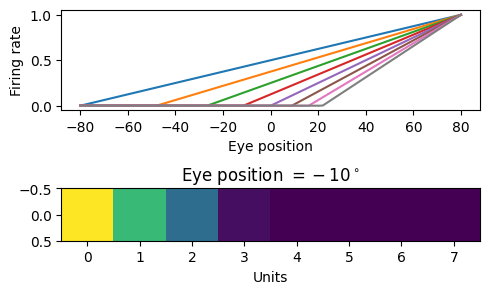
\includegraphics[scale=0.8, max width=\linewidth]{./fig/solve-credit-assignment-problem/backpropagation/cell032.png}
	\caption{cell032.png}
	\label{cell032.png}
\end{figure}

\section{神経サンプリング}
サンプリングに基づく符号化(sampling-based coding; SBC or neural sampling model)をガウス尺度混合モデルを例にとり実装する.
\subsection{ガウス尺度混合モデル}
\textbf{ガウス尺度混合 (Gaussian scale mixture; GSM) モデル}\index{がうすしゃくどこんごう (Gaussian scale mixture; GSM) もでる@ガウス尺度混合 (Gaussian scale mixture; GSM) モデル}は確率的生成モデルの一種である\citep{Wainwright1999-cl}\citep{Orban2016-tm}.GSMモデルでは入力を次式で予測する:
\begin{equation}
\text{入力}={z}\left(\sum \text{神経活動} \times \text{基底} \right) + \text{ノイズ}
\end{equation}
前節までのスパース符号化モデル等と同様に,入力が基底の線形和で表されるとしている.ただし,尺度(scale)パラメータ$z$が基底の線形和に乗じられている点が異なる.\footnote{コードは\citep{Orban2016-tm} \url{https://github.com/gergoorban/sampling_in_gsm}, および\citep{Echeveste2020-sh} \url{https://bitbucket.org/RSE_1987/ssn_inference_numerical_experiments/src/master/}を参考に作成した.}
\subsubsection{事前分布}
$\mathbf{x} \in \mathbb{R}^{N_x}$, $\mathbf{A} \in \mathbb{R}^{N_x\times N_y}$, $\mathbf{y} \in \mathbb{R}^{N_y}$, $\mathbf{z} \in \mathbb{R}$とする.
\begin{equation}
p\left(\mathbf{x}\mid\mathbf{y}, z\right)=\mathcal{N}\left(z \mathbf{A} \mathbf{y}, \sigma_{\mathbf{x}}^{2} \mathbf{I}\right)
\end{equation}
事前分布を
\begin{align}
p\left(\mathbf{y}\right)&=\mathcal{N}\left(\mathbf{0}, \mathbf{C}\right)\\
p\left(z\right)&=\Gamma (k, \vartheta)
\end{align}
とする.$\Gamma(k, \vartheta)$はガンマ分布であり,$k$は形状(shape)パラメータ,$\vartheta$は尺度(scale)パラメータである.$p\left(\mathbf{y}\right)$は$\mathbf{y}$の事前分布であり,刺激がない場合の自発活動の分布を表していると仮定する.
\subsubsection{重み行列$\mathbf{A}$の作成}
\begin{lstlisting}[language=julia]
using PyPlot, LinearAlgebra, Random, Distributions, KernelDensity, StatsBase
using PyPlot: matplotlib
Random.seed!(0)
rc("axes.spines", top=false, right=false)
\end{lstlisting}
\begin{lstlisting}[language=julia]
function gabor(x, y, θ, σ=1, λ=2, ψ=0)
    xθ = x * cos(θ) + y * sin(θ)
    yθ = -x * sin(θ) + y * cos(θ)
    return exp(-.5(xθ^2 + yθ^2)/σ^2) * cos(2π/λ * xθ + ψ)
end;
\end{lstlisting}
\begin{lstlisting}[language=julia]
function get_A(WH, Ny)
    Nx = WH^2
    A = zeros(Nx, Ny) # weight matrix
    p = range(-3, 3, length=WH) # position
    θ = (1:Ny) / Ny * π # theta for gabor
    for i in 1:Ny
        gb = gabor.(p', p, θ[i])
        gb /= norm(gb) + 1e-8 # normalization
        A[:, i] = gb[:] # flatten and save
    end
    return A
end;
\end{lstlisting}
\begin{lstlisting}[language=julia]
WH = 16   # width/height of input image
Nx = WH^2 # dimension of the observed variable x
Ny = 50  # dimension of the hidden variable y

A = get_A(WH, Ny);
\end{lstlisting}
重み行列$\mathbf{A}$の一部を描画してみよう.
\begin{lstlisting}[language=julia]
figure(figsize=(2,2))
plot_idx = [2,4,6,8]
weight_idx = [37,25,50,13]
titles = ["", "0°", "±90°", ""]
for i in 1:4
    subplot(3,3,plot_idx[i])
    title(titles[i])
    imshow(reshape(A[:, weight_idx[i]], WH, WH), cmap="gray")
    axis("off")
end
subplots_adjust(wspace=0.01, hspace=0.01)
\end{lstlisting}
\begin{figure}[ht]
	\centering
	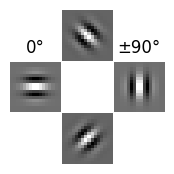
\includegraphics[scale=0.8, max width=\linewidth]{./fig/bayesian-brain/neural-sampling/cell007.png}
	\caption{cell007.png}
	\label{cell007.png}
\end{figure}
\subsubsection{分散共分散行列$\mathbf{C}$の作成}
$\mathbf{C}$は$y$の事前分布の分散共分散行列である.\citep{Orban2016-tm}では自然画像を用いて作成しているが,ここでは簡単のため$\mathbf{A}$と同様に\citep{Echeveste2020-sh}に従って作成する.前項で作成した通り,$\mathbf{A}$の各基底には周期性があるため,類似した基底を持つニューロン同士は類似した出力をすると考えられる.Echevesteらは$\theta\in[-\pi/2, \pi/2)$の範囲においてFourier基底を複数作成し,そのグラム行列(Gram matrix)を係数倍したものを$\mathbf{C}$と設定している.ここではガウス過程(Gaussian process)モデルとの類似性から,周期カーネル(periodic kernel) 
\begin{equation}
K(\theta, \theta')=\exp\left[\phi_1 \cos \left(\dfrac{|\theta-\theta'|}{\phi_2}\right)\right]
\end{equation}
を用いる.ここでは$|\theta-\theta'|=m\pi\ (m=0,1,\ldots)$の際に類似度が最大になればよいので,$\phi_2=0.5$とする.これが正定値行列になるように単位行列の係数倍$\epsilon\mathbf{I}$を加算し,スケーリングした上で,\jl{Symmetric(C)}や\jl{Matrix(Hermitian(C)))}により実対象行列としたものを$\mathbf{C}$とする.$\mathbf{C}$を正定値行列にする理由はJuliaの\jl{MvNormal}がCholesky分解を用いて多変量正規分布の乱数を生成するためである. 事前に\jl{cholesky(C)}が実行できるか確認するのもよい.
\begin{lstlisting}[language=julia]
function get_C(Ny, C_range=[-0.5, 4.0], eps=0.1, ψ₁=2.0, ψ₂=0.5)
    K(x₁, x₂, ψ₁, ψ₂) = exp(ψ₁ * cos(abs(x₁-x₂) / ψ₂)) # periodic kernel
    θ = (1:Ny) / Ny * π # theta for gabor
    C = K.(θ', θ, ψ₁, ψ₂) # create covariance matrix
    C += eps * I # regularization to make C positive definite
    C_min, C_max = minimum(C), maximum(C)
    C = C_range[1] .+ (C_range[2]-C_range[1]) * (C .- C_min) / (C_max - C_min)
    return Symmetric(C); # make symmetric matrix using upper triangular matrix
end;
\end{lstlisting}
\begin{lstlisting}[language=julia]
C = get_C(Ny)

figure(figsize=(3,2))
title(L"$\mathbf{C}$")
ims = imshow(C, origin="lower", cmap="bwr", vmin=-4, vmax=4, extent=(-90, 90, -90, 90))
xticks([-90,0,90]); yticks([-90,0,90]); 
xlabel(L"$\theta$ (Pref. ori)"); ylabel(L"$\theta$ (Pref. ori)")
colorbar(ims);
tight_layout()
\end{lstlisting}
\begin{figure}[ht]
	\centering
	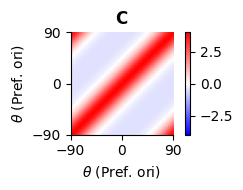
\includegraphics[scale=0.8, max width=\linewidth]{./fig/bayesian-brain/neural-sampling/cell010.png}
	\caption{cell010.png}
	\label{cell010.png}
\end{figure}
ここでPref. oriは最適方位 (preferred orientation)を意味する.
\subsubsection{事後分布の計算}
事後分布は$z$と$\mathbf{y}$のそれぞれについて次のように求められる.
\begin{align}
p(z \mid \mathbf{x}) &\propto p(z) \mathcal{N}\left(0, z^{2} \mathbf{A C A}^{\top}+\sigma_{x}^{2} \mathbf{I}\right)\\
p(\mathbf{y} \mid z, \mathbf{x})& = \mathcal{N}\left(\mu(z, \mathbf{x}), \Sigma(z)\right)
\end{align}
ただし,
\begin{align}
\Sigma(z)&=\left(\mathbf{C}^{-1}+\frac{z^{2}}{\sigma_{x}^{2}} \mathbf{A}^{\top} \mathbf{A}\right)^{-1}\\
\mu(z, \mathbf{x})&=\frac{z}{\sigma_{x}^{2}} \Sigma(z) \mathbf{A}^{\top} \mathbf{x}
\end{align}
である.
最終的な予測において$z$の事後分布は必要でないため,$p(\mathbf{y} \mid z, \mathbf{x})$から$z$を消去することを考えよう.厳密に行う場合,次式のように周辺化(marginalization)により,$z$を (積分) 消去する必要がある.
\begin{equation}
p(\mathbf{y} \mid \mathbf{x}) = \int dz\ p(z\mid \mathbf{x})\cdot p(\mathbf{y} \mid z, \mathbf{x})
\end{equation}
周辺化においては,まず$z$のMAP推定 (最大事後確率推定) 値 $z_{\mathrm{MAP}}$を求める.
\begin{equation}
z_{\mathrm{MAP}} = \underset{z}{\operatorname{argmax}} p(z\mid \mathbf{x})
\end{equation}
次に$z_{\mathrm{MAP}}$の周辺で$p(z\mid \mathbf{x})$を積分し,積分値が一定の閾値を超える$z$の範囲を求め,この範囲で$z$を積分消去してやればよい.しかし,$z$は単一のスカラー値であり,この手法で推定するのは煩雑であるために近似手法が\citep{Echeveste2017-wu}において提案されている.Echevesteらは第一の近似として,$z$の分布を$z_{\mathrm{MAP}}$でのデルタ関数に置き換える,すなわち,$p(z\mid \mathbf{x})\simeq \delta (z-z_{\mathrm{MAP}})$とすることを提案している.この場合,$z$は定数とみなせ,$p(\mathbf{y} \mid \mathbf{x})\simeq p(\mathbf{y} \mid \mathbf{x}, z=z_{\mathrm{MAP}})$となる.第二の近似として,$z_{\mathrm{MAP}}$を真のコントラスト$z^*$で置き換えることが提案されている.GSMへの入力$\mathbf{x}$は元の画像を$\mathbf{\tilde x}$とすると,$\mathbf{x}=z^* \mathbf{\tilde x}$としてスケーリングされる.この入力の前処理の際に用いる$z^*$を用いてしまおうということである.この場合,$p(\mathbf{y} \mid \mathbf{x})\simeq p(\mathbf{y} \mid \mathbf{x}, z=z^*)$となる.しかし,入力を任意の画像とする場合,$z^*$は未知である.簡便さと精度のバランスを取り,ここでは第一の近似,$z=z_{\mathrm{MAP}}$とする手法を用いることにする.
\begin{lstlisting}[language=julia]
# log pdf of p(z)
log_Pz(z, k, θ) = logpdf.(Gamma(k, θ), z)

# pdf of p(z|x)
function Pz_x(z_range, x, ACAᵀ, σₓ², k, θ)
    n_contrasts = length(z_range)
    log_p = zeros(n_contrasts)
    μxz = zeros(size(x))
    dz = z_range[2] - z_range[1]
    for i in 1:n_contrasts
        Cxz = z_range[i]^2 * ACAᵀ + σₓ² * I
        log_p[i] = log_Pz(z_range[i], k, θ) + logpdf(MvNormal(μxz, Symmetric(Cxz)), x)
    end
    p = exp.(log_p .- maximum(log_p)) # for numerical stability
    p /= sum(p) * dz
    return p
end;
\end{lstlisting}
\begin{lstlisting}[language=julia]
# mean and covariance matrix of p(y|x, z)
function post_moments(x, z, σₓ², A, AᵀA, C⁻¹)
    Σz = inv(C⁻¹ + (z^2 / σₓ²) * AᵀA)
    μzx = (z/σₓ²) * Σz * A' * x
    return μzx, Σz
end;
\end{lstlisting}
\subsubsection{シミュレーション}
\begin{lstlisting}[language=julia]
AᵀA = A' * A
ACAᵀ = A * C * A'

σₓ = 1.0 # Noise of the x process
σₓ² = σₓ^2
k, θ = 2.0, 2.0 # Parameter of the gamma dist. for z (Shape, Scale)

C⁻¹ = inv(C); # inverse of C
\end{lstlisting}
入力データの作成
\begin{lstlisting}[language=julia]
Z = [0.0, 0.25, 0.5, 1.0, 2.0] # true contrasts z^*
n_samples = size(Z)[1]
y = rand(MvNormal(zeros(Ny), C), 1) # sampling from P(y)=N(0, C)
X = stack([rand(MvNormal(vec(z*A*y), σₓ*I)) for z in Z])';
\end{lstlisting}
\begin{lstlisting}[language=julia]
x_min, x_max = minimum(X), maximum(X)

figure(figsize=(4,2))
for s in 1:n_samples
    subplot(1, n_samples, s)
    title(L"$z$: "*string(Z[s]))
    imshow(reshape(X[s, :], WH, WH), vmin=x_min, vmax=x_max, cmap="gray")
    axis("off")
end
tight_layout()
\end{lstlisting}
\begin{figure}[ht]
	\centering
	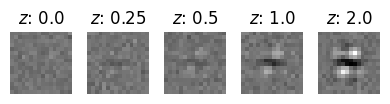
\includegraphics[scale=0.8, max width=\linewidth]{./fig/bayesian-brain/neural-sampling/cell019.png}
	\caption{cell019.png}
	\label{cell019.png}
\end{figure}
事後分布の計算をする.
\begin{lstlisting}[language=julia]
μ_post = zeros(n_samples, Ny)
σ_post = zeros(n_samples, Ny)
Σ_post = zeros(n_samples, Ny, Ny)

z_range = range(0, 5.0, length=100) # range of z for MAP estimation
Z_MAP = zeros(n_samples) 

for s in 1:n_samples
    p_z = Pz_x(z_range, X[s, :], ACAᵀ, σₓ², k, θ)
    Z_MAP[s] = z_range[argmax(p_z)] # MAP estimated z
    μ_post[s, :], Σ_post[s, :, :] = post_moments(X[s, :], Z_MAP[s], σₓ², A, AᵀA, C⁻¹)
    σ_post[s, :] = sqrt.(diag(Σ_post[s, :, :]))
end
\end{lstlisting}
\subsubsection{結果}
\begin{lstlisting}[language=julia]
θs = range(-90, 90, length=Ny)
cm = get_cmap(:Greens) # get color map
cms = cm.((1:n_samples)/n_samples) # color list

fig, ax = subplots(1, 3, figsize=(7.5, 2))
ax[1].scatter(Z, Z_MAP, c=cms)
ax[1].plot(Z, Z_MAP, color="tab:gray", zorder=0)
ax[1].set_xlabel(L"$z$"); ax[1].set_ylabel(L"$z_{MAP}$"); 
for s in 1:n_samples
    ax[2].plot(θs, μ_post[s, :], color=cms[s])
    ax[3].plot(θs, σ_post[s, :], color=cms[s], label=L"$z$ : "*string(Z[s]))
end
ax[2].set_ylabel(L"$\mu$"); ax[3].set_ylabel(L"$\sigma$")
for i in 2:3
    ax[i].set_xticks([-90,0,90])
    ax[i].set_xlabel(L"$\theta$ (Pref. ori)")
end
ax[3].legend(bbox_to_anchor=(1.05, 1), loc="upper left", borderaxespad=0)
tight_layout()
\end{lstlisting}
\begin{figure}[ht]
	\centering
	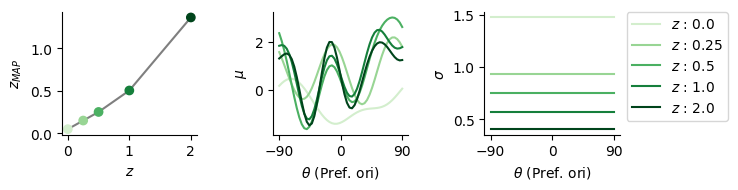
\includegraphics[scale=0.8, max width=\linewidth]{./fig/bayesian-brain/neural-sampling/cell023.png}
	\caption{cell023.png}
	\label{cell023.png}
\end{figure}
\begin{lstlisting}[language=julia]
fig, ax = subplots(1, n_samples, figsize=(7.5, 1), sharex="all", sharey="all")
for s in 1:n_samples
    ax[s].set_title(L"$z$ : "*string(Z[s]))
    ims = ax[s].imshow(Σ_post[s, :, :], origin="lower", cmap="bwr", extent=(-90, 90, -90, 90), vmin=-1, vmax=1)
    ax[s].set_xticks([-90,0,90]); ax[s].set_yticks([-90,0,90]);
    if s == 1
        ax[s].set_ylabel(L"$\theta$ (Pref. ori)")
    elseif s == ceil(Int, n_samples/2) 
        ax[s].set_xlabel(L"$\theta$ (Pref. ori)"); 
    end
end
fig.colorbar(ims, ax=ax[n_samples]);
\end{lstlisting}
\begin{figure}[ht]
	\centering
	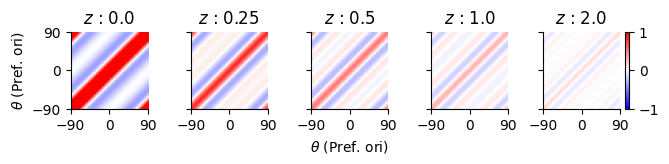
\includegraphics[scale=0.8, max width=\linewidth]{./fig/bayesian-brain/neural-sampling/cell024.png}
	\caption{cell024.png}
	\label{cell024.png}
\end{figure}
\subsubsection{出力のサンプリング}
\begin{lstlisting}[language=julia]
membrane_potential(y, α=2.4, β=1.9, γ=0.6) = α * max(0, y+β)^γ
\end{lstlisting}
事後分布から応答をサンプリングする.
\begin{lstlisting}[language=julia]
nt = 1000
h_gsm = zeros(n_samples, Ny, nt)
for s in 1:n_samples
    μ = μ_post[s, :]
    Σ = Σ_post[s, :, :]
    sample = rand(MvNormal(μ, Symmetric(Σ)), nt)
    h_gsm[s, :, :] = membrane_potential.(sample)
end
\end{lstlisting}
\begin{lstlisting}[language=julia]
# modified from https://matplotlib.org/stable/gallery/statistics/confidence_ellipse.html
function confidence_ellipse(x, y, ax, n_std=3, alpha=1, facecolor="none", edgecolor="tab:gray")
    pearson = cor(x,y)
    rx, ry = sqrt(1 + pearson), sqrt(1 - pearson)
    ellipse = matplotlib.patches.Ellipse((0, 0), width=2*rx, height=2*ry, alpha=alpha, 
        fc=facecolor, ec=edgecolor, lw=2, zorder=0)
    scales = [std(x), std(y)] * n_std
    means = [mean(x), mean(y)]
    transf = matplotlib.transforms.Affine2D().rotate_deg(45).scale(scales...).translate(means...)
    ellipse.set_transform(transf + ax.transData)
    return ax.add_patch(ellipse)
end;
\end{lstlisting}
\begin{lstlisting}[language=julia]
fig, ax = subplots(figsize=(4, 3))
unit_idx = [1, 25]
for s in 1:n_samples
    h₁, h₂ = h_gsm[s, unit_idx[1], :], h_gsm[s, unit_idx[2], :]
    ax.plot(h₁[1:15], h₂[1:15], marker="o", markersize=5, alpha=0.5, color=cms[s], label=L"$z$ : "*string(Z[s]))
    confidence_ellipse(h₁, h₂, ax, 3, 1, "none", cms[s])
end
ax.set_xlabel("Neuron #"*string(unit_idx[1])); ax.set_ylabel("Neuron #"*string(unit_idx[2]))
axins = [ax.inset_axes([0.85, -0.25,0.15,0.15]), ax.inset_axes([-0.3,0.85,0.15,0.15])]
for i in 1:2
    axins[i].imshow(reshape(A[:,unit_idx[i]], WH, WH), cmap="gray")
    axins[i].axis("off")
end
ax.set_aspect("equal", "box")
ax.legend(bbox_to_anchor=(1.05, 1), loc="upper left", borderaxespad=0)
tight_layout()
\end{lstlisting}
\begin{figure}[ht]
	\centering
	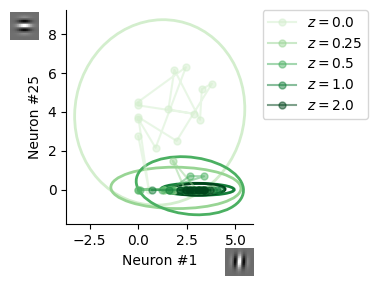
\includegraphics[scale=0.8, max width=\linewidth]{./fig/bayesian-brain/neural-sampling/cell030.png}
	\caption{cell030.png}
	\label{cell030.png}
\end{figure}
\subsection{興奮性・抑制性神経回路によるサンプリング}
前節で実装したMCMCを\textbf{興奮性・抑制性神経回路 (excitatory-inhibitory (E-I) network)}\index{こうふんせい・よくせいせいしんけいかいろ (excitatory-inhibitory (E-I) network)@興奮性・抑制性神経回路 (excitatory-inhibitory (E-I) network)} で実装する.HMCとLMCの両方を神経回路で実装する.
Hamiltonianを用いる場合,一般化座標$\mathbf{q}$を興奮性神経細胞の活動$\mathbf{u}$, 一般化運動量$\mathbf{p}$を抑制性神経細胞の活動$\mathbf{v}$に対応させる.ToDo: 詳しい説明.
簡単のため,前項で用いた入力刺激のうち,最も$z$が大きいサンプルのみを使用する.
\begin{lstlisting}[language=julia]
dt = 1e-2 # ms
τ, τl = 10.0, 150.0 # ms
α_in = [1/τ - 1/τl, 1/τ + 1/τl]
α_ext = [1/τl, -1/τ]
ρ = sqrt(2*dt/τl);

nt = 50000
M = cat(ones(1,1), C; dims=(1,2));
x_idx = n_samples # get last x
x = X[x_idx, :]
u_init = [1; zeros(Ny)];
\end{lstlisting}
\begin{lstlisting}[language=julia]
function ∇ᵤlogP(u, x, σₓ², A, C⁻¹)
    z, y = abs(u[1]), u[2:end]
    pred_error = A' * (x - z*A*y) / σₓ² # prediction error signal
    du = zeros(size(u))
    du[1] = sign(u[1]) * (y' * pred_error - z)
    du[2:end] = z * pred_error - C⁻¹*y
    return du
end
\end{lstlisting}
\begin{lstlisting}[language=julia]
∇log_p(u) = ∇ᵤlogP(u, x, σₓ², A, C⁻¹);
\end{lstlisting}
\begin{lstlisting}[language=julia]
function neural_lmc(∇log_p::Function, u_init::Vector{Float64}, α::Float64, ρ::Float64, dt::Float64, nt::Int)
    d = length(u_init)
    u = zeros(nt, d)
    u[1, :] = u_init

    for t in 1:nt-1
        I_ext = ∇log_p(u[t, :]) # external input
        u[t+1, :] = u[t, :] + dt * (α * I_ext) + ρ * randn(d) 
    end
    return u
end

function neural_hmc(∇log_p::Function, u_init::Vector{Float64}, M::Matrix{Float64}, 
        α_in::Vector{Float64}, α_ext::Vector{Float64}, ρ::Float64, dt::Float64, nt::Int)
    d = length(u_init)
    u, v = zeros(nt, d), zeros(nt, d)
    u[1, :] = u_init

    for t in 1:nt-1
        I_ext = ∇log_p(u[t, :]) # external input
        I_in = M * (u[t, :] - v[t, :]) # internal input
        u[t+1, :] = u[t, :] + dt * (α_in[1] * I_in + α_ext[1] * I_ext) + ρ * randn(d) 
        v[t+1, :] = v[t, :] + dt * (α_in[2] * I_in + α_ext[2] * I_ext) + ρ * randn(d)
    end
    return u, v
end;
\end{lstlisting}
\begin{lstlisting}[language=julia]
@time u_nlmc = neural_lmc(∇log_p, u_init, α_ext[1], ρ, dt, nt);
\end{lstlisting}
\begin{lstlisting}[language=julia]
@time u_nhmc, v_nhmc = neural_hmc(∇log_p, u_init, M, α_in, α_ext, ρ, dt, nt);
\end{lstlisting}
初めの100msはburn-in期間として除く.またダウンサンプリングする.
\begin{lstlisting}[language=julia]
L = 100
burn_in = 10000
mcmc_time = (burn_in*dt):(L*dt):(nt*dt); # time for plot
\end{lstlisting}
\begin{lstlisting}[language=julia]
mean_nlmc = mean(u_nlmc[burn_in:L:end, 2:end], dims=2); # pseudo-LFP
mean_nhmc = mean(u_nhmc[burn_in:L:end, 2:end], dims=2);

autocorr_nlmc = autocor(mean_nlmc, 1:length(mean_nlmc)-1);
autocorr_nhmc = autocor(mean_nhmc, 1:length(mean_nhmc)-1);
\end{lstlisting}
$z$の推定過程を描画する.また,$z$を除いた$\mathbf{u}$を平均化し,自己相関の度合いを確認する.
\begin{lstlisting}[language=julia]
fig, ax = subplots(1,2,figsize=(6,2.5),sharex="all")
ax[1].plot(mcmc_time, u_nhmc[burn_in:L:end, 1], color="tab:red")
ax[1].plot(mcmc_time, u_nlmc[burn_in:L:end, 1], color="tab:blue")
ax[1].axhline(Z[x_idx], linestyle="dashed", color="tab:gray", alpha=0.5)
ax[1].set_xlabel("Time (ms)"); ax[1].set_ylabel(L"Estimated $z$")
ax[1].set_xlim(mcmc_time[1], mcmc_time[end])

ax[2].plot(mcmc_time[1:end-1], autocorr_nhmc, color="tab:red", label="Hamiltonian")
ax[2].plot(mcmc_time[1:end-1], autocorr_nlmc, color="tab:blue", label="Langevin")
ax[2].set_xlabel("Time (ms)"); ax[2].set_ylabel("Autocorrelation")
ax[2].set_xlim(mcmc_time[1], mcmc_time[end])
ax[2].axhline(0, linestyle="dashed", color="tab:gray", alpha=0.5)
ax[2].legend()
fig.tight_layout()
\end{lstlisting}
\begin{figure}[ht]
	\centering
	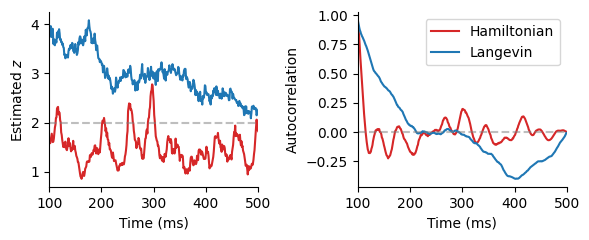
\includegraphics[scale=0.8, max width=\linewidth]{./fig/bayesian-brain/neural-sampling/cell042.png}
	\caption{cell042.png}
	\label{cell042.png}
\end{figure}
Hamiltonianネットワークは自己相関を振動により低下させることで,効率の良いサンプリングを実現している.ToDo: 普通にMCMCやる場合も自己相関は確認したほうがいいという話をどこかに書く.
推定された事後分布を特定の神経細胞のペアについて確認する.
\begin{lstlisting}[language=julia]
h_nhmc = membrane_potential.(u_nhmc[burn_in:L:end, :])
h_nlmc = membrane_potential.(u_nlmc[burn_in:L:end, :])

kde_bound = ((-3,5),(0,8)) # ((xlo,xhi),(ylo,yhi))
U_gsm = kde((h_gsm[x_idx, unit_idx[1], :], h_gsm[x_idx, unit_idx[2], :]), boundary=kde_bound)
U_nhmc = kde((h_nhmc[:, unit_idx[1]+1], h_nhmc[:, unit_idx[2]+1]), boundary=kde_bound)
U_nlmc = kde((h_nlmc[:, unit_idx[1]+1], h_nlmc[:, unit_idx[2]+1]), boundary=kde_bound);
\end{lstlisting}
\begin{lstlisting}[language=julia]
fig, ax = plt.subplots(1,3, figsize=(6, 2.5), sharey="all", sharex="all")
ax[1].contourf(U_gsm.x, U_gsm.x, U_gsm.density)
ax[1].set_title("Actual")
ax[2].contourf(U_nhmc.x, U_nhmc.x, U_nhmc.density)
ax[2].set_title("Hamiltonian")
ax[3].contourf(U_nlmc.x, U_nlmc.x, U_nlmc.density)
ax[3].set_title("Langevin")
ax[1].set_ylabel("Neuron #"*string(unit_idx[2]))
ax[2].set_xlabel("Neuron #"*string(unit_idx[1])) 
fig.tight_layout()
\end{lstlisting}
\begin{figure}[ht]
	\centering
	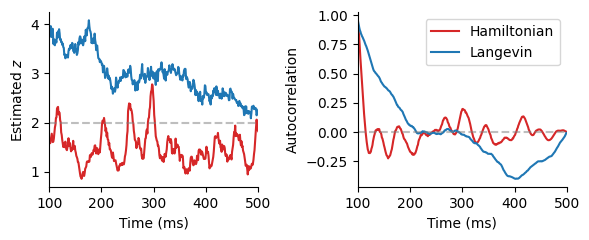
\includegraphics[scale=0.8, max width=\linewidth]{./fig/bayesian-brain/neural-sampling/cell045.png}
	\caption{cell045.png}
	\label{cell045.png}
\end{figure}
Hamiltonianネットワークの方が安定して事後分布を推定することができている.ToDo: 以下の記述.ここでは重みを設定したが, \citep{Echeveste2020-sh}ではRNNにBPTTで重みを学習させている.動的な入力に対するサンプリング \citep{Berkes2011-xj}.burn-inがなくなり効率良くサンプリングできる.
\subsection{Spikingニューラルネットワークにおけるサンプリング}
前項で挙げた例は発火率モデルであったが,SNNにおいてサンプリングを実行する機構自体は考案されている.ToDo: 以下の記述.\citep{Buesing2011-dm}\citep{Masset2022-wh}\citep{Zhang2022-bl}
\subsection{シナプスサンプリング}
ここまでシナプス結合強度は変化せず,神経活動の変動によりサンプリングを行うというモデルについて考えてきた.一方で,シナプス結合強度自体が短時間で変動することによりベイズ推論を実行するというモデルがあり,\textbf{シナプスサンプリング(synaptic sampling)}\index{しなぷすさんぷりんぐ(synaptic sampling)@シナプスサンプリング(synaptic sampling)} と呼ばれる.ToDo: 以下の記述.\citep{Kappel2015-kq}\citep{Aitchison2021-wo}

\end{document}